\documentclass[12pt]{article}
\usepackage{graphicx,indentfirst}
\usepackage{amsmath}
\usepackage{parskip}
\usepackage{float}
\usepackage{amssymb}
%\usepackage{textgreek}
\usepackage{ulem}
\usepackage{tikz}
\usepackage{ marvosym }
\usepackage{ scrextend }
\usepackage{ setspace }


%\usepackage{showframe}

\pagestyle{plain}
\baselineskip 18pt
\textwidth 6.5in
\textheight 7.8in
\oddsidemargin 0.1in
\evensidemargin 0.1in
\topmargin 0.3in

\newcommand{\be}{\begin{equation}}
\newcommand{\ee}{\end{equation}}
\newcommand{\reff}[1]{(\ref{#1})}
\newcommand{\problem}[2]{\vspace{1em} \textbf{#1:} \\ {#2}}
\newcommand{\dd}{\mathrm{d}}
\newcommand{\tbs}{\textbackslash{}}

\usepackage{datetime}
\newdateformat{properdate}{\THEDAY{}\;\monthname[\THEMONTH]{}\;\THEYEAR}

% \problem{Name}{Text}
% \fbox{ text-to-be-outlined }

\begin{document}

\title{\vspace{-5em}How to \LaTeX}
\author{George Wong, David Mykytyn}
\date{\properdate\today}
\maketitle

\vspace{1em}

\section{What is \LaTeX?}
\begin{itemize}
\item Used in textbooks, journal/conference articles, and lab reports!
\item You provide the material and \LaTeX\ renders according to typographical conventions \&c.
\item Not a WYSIWYG (what you see is what you get) editor!
\item Initial release 1985 by Leslie Lamport -- \underline{La}mport \TeX. \TeX\ originally from Donald Knuth in 1978.\footnote{Knuth says to pronounce his name ``Ka-NOOTH''. See {\tt{}http://www-cs-faculty.stanford.edu/\textasciitilde{}uno/faq.html}}
\item \TeX\ should be pronounced as ``tech'' in \emph{technical}. %\tau\epsilon\chi\nu\eta
\end{itemize}

\section{\LaTeX\ rendering tools}
\begin{itemize}
\item In ye olde days, used the {\tt tex} command from the command line -- produced postscript {\tt .ps} file. Now straight to {\tt .pdf} with many tools!
\item OSX
\begin{itemize}
\item TeXworks
\item MacTeX
\end{itemize}
\item Windows
\begin{itemize}
\item MiKTeX
\end{itemize}
\item Linux
\begin{itemize}
\item Google is your friend! Personally I use {\tt vim} (but you can use any text editor) with {\tt pdflatex}.
\end{itemize}
\item Alternatively, use an online service like
\begin{itemize}
\item https://www.overleaf.com/
\item https://www.sharelatex.com/
\end{itemize}
Some services might even allow you to collaborate (useful for partner lab reports!)
\end{itemize}

\section{Document structure}
\LaTeX\ expects a specific structure to your document. Generally, the document is in two parts, a \textbf{preamble} and a \textbf{body}. In the preamble, you tell the renderer what sort of document this is (books look different than journal articles), along with what extra \emph{package}s to include, e.g., Greek or special math characters. The ``meat'' of your document---everything that you want to actually show up---goes in the body.

Here's an example document:

\begin{addmargin}[1em]{0em}
\begin{verbatim}
\documentclass[12pt]{article}
\usepackage{amsmath}
\usepackage{amssymb}

\begin{document}
\section{Section the First}
Lorem ipsum dolor sit amet, quo autem fugit vivendum eu, mel at 
lorem homero hendrerit
\end{document}
\end{verbatim}
\end{addmargin}

The first line tells the renderer to treat the document as an \emph{article} and to normalize to 12 pt font. The next two lines are my personal ``always-use'' packages. They provide various math symbols and environments that I find interminably useful.

The rest of the document lies with the {\tt document} environment, enclosed by the {\tt \tbs begin\{$\cdot$\}} and {\tt \tbs end\{$\cdot$\}} tags. You can divide your document into sections, using {\tt \tbs section \{$\cdot$\}} and even {\tt \tbs subsection} and even even {\tt \tbs subsubsection}. \LaTeX will automatically number your sections and subsections for you.

\section{Styling}
In general, you try to avoid explicitly styling your document as much as possible. The renderer almost definitely knows better than you. Styling font, e.g., adding emphasis, is fine though.

\begin{center}
\begin{tabular}{l l}
Product & Code \\
\hline
\emph{Your text here!} & {\tt \tbs{}emph\{Your text here!\}} \\
\textbf{Your text here!} & {\tt \tbs{}textbf\{Your text here!\}} \\
\underline{Your text here!} & {\tt \tbs{}underline\{Your text here!\}}
\end{tabular}
\end{center}

When it's \textbf{\emph{absolutely}} necessary, you can add spaces, carriage returns, and page breaks
\begin{center}
\begin{tabular}{l l}
Effect & Code \\
\hline
Narrow space & {\tt \tbs{},} \\
Em-width space & {\tt \tbs } \;\;followed by space \\
Wide space & {\tt \tbs{};} \\
``Backwards'' space & {\tt \tbs{}! }\\
Single line break / carriage return & {\tt \tbs\tbs} \\
Four-line break & {\tt \tbs{}vspace\{4em\}} \\
Page break & {\tt \tbs{}vfill} \\
Fill extra horizontal space & {\tt \tbs{}hfill}
\end{tabular}
\end{center}

You've noticed by now that commands seem to be preceded by the backslash {\tt \tbs} character. The backslash is called an \emph{escape} character. Using it lets the compiler know that it should treat the following characters a part of a command as opposed to normal text. 

\section{Labels}
Labels allow you to reference parts of the document (such as images / equations) by number without requiring you to keep a list yourself.
[TODO]


\section{Math mode}
Equations are written in a special ``math mode'' In math mode, there are extra commands that work to produce mathematical symbols, for instance \begin{verbatim}$\alpha$\end{verbatim} will produce $\alpha$, or whatever combinations your heart desires. Notice the {\$} are used to encase something to be used inline. If you want to have something on a separate line, and numbered, you should use the command {\tt \tbs begin\{equation\}} and end it similarily. 
\begin{itemize}
\item \tbs{}usepackage\{amsmath\}

\item \tbs{}usepackage\{amssymb\}

\item To get a superscript, use a carot ``{\tt \^{}}'', and for subscript use an underscore ``{\tt \_{}}''. Note that if there is only one character or command in the super(sub)script, than there is no need to use brackets, but if you want multiple characters to be super(sub)scripted, you have to encase them in curly-brackets. e.g. $10^{10^{100}}$ which is produced by \begin{verbatim}$10^{10^{100}}$\end{verbatim}

\item \tbs{}sqrt $\sqrt{1+x^2}$

\item \tbs{}int $\int_0^\infty \mathrm{e}^{\frac{-x^2}{2}} \mathrm{d}x$ Note also {\tt \tbs iint} and {\tt \tbs iiint} provide double and triple integrals respectively.

\item special sequences \\sin You shouldn't write out ``sin'' or etc., instead you should use the provided functions {\tt \tbs sin\{\ldots\}} and same for other common functions such as exp, log, or whatever.

\item Styling fractions as $x$ over $y$ can be done with the {\tt \tbs frac} and {\tt \tbs dfrac} commands. The form of each command is {\tt \tbs frac\{x\}\{y\}} where {\tt x} is what you want to appear in the numerator and {\tt y} is what you want to appear in the denominator.

The latter of the two, {\tt \tbs dfrac} puts the renderer into \textbf{display} mode, which generally expands the fraction, making the text larger. Compare 

$\frac{x}{y}$ vs $\dfrac{x}{y}$

The version on the left uses the {\tt \tbs frac} command; the version on the right uses {\tt \tbs dfrac}.
\item \tbs{}left and \tbs{right} If you want to make sure that your parenthesis are scaled appropriately to whatever sized math is encased in them, use \tbs left( and \tbs right). For an example, see $(\dfrac{\sum_{n=0}^{100} \frac{1}{n^2}}{2})$ versus $\left(\dfrac{\sum_{n=0}^{100} \frac{1}{n^2}}{2}\right)$

\item \tbs{}mathrm 

\item \tbs{}mathbb

\item \tbs{}mathcal
\item putting spaces in math mode
\item  - align
\item - array
\end{itemize}
 
\section{Detexify}
This tool deserves its own section
Detexify {\tt http://detexify.kirelabs.org/}

\section{Lists}

\section{Floats}
Floats are a special type of environment that indicates to the renderer that the contained elements should all be displayed on one page. They should be used for things like tables and plots, which often include titles and captions that should not be spread over multiple pages.

Because floats may not be able to be placed exactly where they appear in the source without breaking the flow of the document, they accept a \textbf{positioning} argument, which is one of {\tt h,t,b,p}, indicating \textbf{\underline{h}ere}, \textbf{\underline{t}op of page}, \textbf{\underline{b}ottom of page}, and \textbf{special \underline{p}age for floats}, respectively. If you include the {\tt float} package, you can also use the capital {\tt H} specifier which overrides all of the renderer's sensibilities and places the figure \textbf{right \underline{H}ere}. 

A bit confusingly, floats are actually named {\tt figure} in the source. Like any other section, they begin and end as

\begin{verbatim}
\begin{figure}[h]
    ... your source here
\end{figure}
\end{verbatim}


\subsection{Tables}

\subsection{Graphics}
\LaTeX\ offers several options for adding graphics to your document. 

The first (and easiest) is to simply include an image file, like a {\tt bmp} or {\tt png}. This can be done using the {\tt \tbs includegraphics} command, formatted as 

{\tt \tbs includegraphics[args]\{filename\} }

The {\tt args} arguments can be used to set properties like the {\tt height=40mm} or {\tt width=60mm} of the image.

As noted above, graphics you include should probably be within the {\tt float} environment. You can mandate {\tt centering} and add {\tt label}s and {\tt caption}s to the object too, as per

\begin{verbatim}
\begin{figure}
  \centering
  \includegraphics[height=35mm]{latex_is_cool.png}
  \caption{\LaTeX is cool!}
  \label{fig:latexiscool}
\end{figure}
\end{verbatim}

The second option for including an image is to draw it within a {\tt tikzpicture} environment. For now, the exact mechanics of using {\tt tikzpicture} is beyond the scope of this document, but see the following example for inspiration

\begin{verbatim}
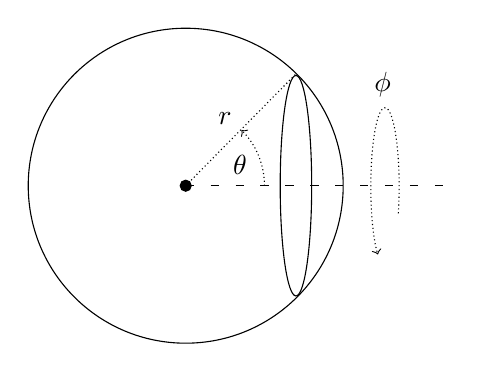
\begin{tikzpicture}
\draw [black] (0,0) circle(2);
\draw [black] (1.4,0) ellipse(0.2 and 1.4);
\draw [loosely dashed] (0,0) -- (3.4,0);
\filldraw[black] (0,0) circle (2pt);
\draw [densely dotted] (0,0) -- (1.4, 1.42);
\draw (0.5, 0.65) node[anchor=south] {$r$};
\draw [densely dotted, ->, xscale=0.18] (15,-0.35) arc (-20:240:1);
\draw (2.5,1) node[anchor=south] {$\phi$};
\draw [densely dotted, ->] (1,0) arc (0:45:1);
\draw (0.9, 0.27) node[anchor=east] {$\theta$};
\end{tikzpicture}
\end{verbatim}

\begin{figure}[H]
\centering
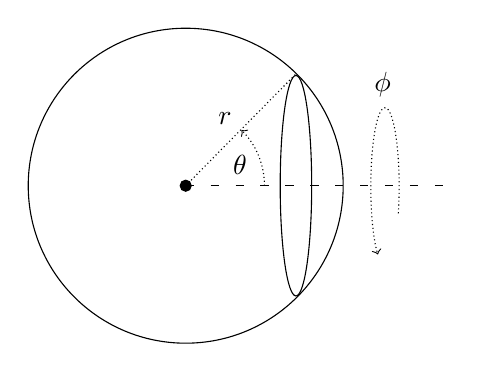
\begin{tikzpicture}
\draw [black] (0,0) circle(2);
\draw [black] (1.4,0) ellipse(0.2 and 1.4);
\draw [loosely dashed] (0,0) -- (3.4,0);
\filldraw[black] (0,0) circle (2pt);
\draw [densely dotted] (0,0) -- (1.4, 1.42);
\draw (0.5, 0.65) node[anchor=south] {$r$};
\draw [densely dotted, ->, xscale=0.18] (15,-0.35) arc (-20:240:1);
\draw (2.5,1) node[anchor=south] {$\phi$};
\draw [densely dotted, ->] (1,0) arc (0:45:1);
\draw (0.9, 0.27) node[anchor=east] {$\theta$};
\end{tikzpicture}
\caption{A {\tt tikz} picture!}
\end{figure}

 
\section{Miscellaneous}

\subsection{Comments}
Use \%

\subsection{How to deal with errors}
Fix them.

\subsection{Quotations}
Note that quotations in LaTeX should be done with two uses of the ```'' key for left hand side and two uses of the ``''' key of the right hand side. This is because you might be used to working with ``smart quotes'' in which left and right quotations marks are done automatically for you, but in LaTeX you have to use separate marks for each quotation. (Note: In a good editor, for instance like {\tt EMACS}, using the quotation key will automatically produce the correct kind if you are in LaTeX-Mode.)

%(Note: In a good editor, for instance like \sout{{\tt EMACS}} a properly-formatted {\tt vim}, using the quotation key will automatically produce the correct kind if you are in LaTeX-Mode)

\subsection{Well wishes}
There's a lot to learn; don't be discouraged! You only need to remember a very small subset of everything in order to produce beautiful documents. Keep templates of useful document classes, look things up (@ Google ``{\tt{}How do I do} X {\tt{}in LaTeX}''), and ask questions when necessary. Learning to write with \LaTeX\ is learning use a new skill. Keep at it and you'll be an expert in no time!




\end{document}
